\chapter{The GAPS experiment} \label{appendixGAPSintro}

%-------------------------------------------------------------------------------
%   The Dark Matter unsolved issue
%-------------------------------------------------------------------------------

\section{The Dark Matter unsolved issue}
\begin{comment}
A wide branch of modern physics is devoted to the study and the understanding of dark
matter. Dark matter is an hypothetical component of the matter, that, unlike the known
matter, does not interact with electromagnetic fields. As a consequence it does not absorb, reflect or emit electromagnetic radiation, making its detection very difficult. This is where the name "dark matter" comes from. The only effects that seem to be related to dark matter are the gravitational types, coming from astrophysical observations. In fact, there are some events that are not explainable by the common theories of gravity accepted by the scientific community, unless there is more matter with respect to what can be detected through all the other physical effects. 
\end{comment}

The study and understanding of dark matter is a broad field of modern physics. Dark matter is a hypothetical component of matter that, unlike known matter, is unaffected by electromagnetic fields. As a result, it does not absorb, reflect, or emit electromagnetic radiation, making it difficult to detect. This is the origin of the term "dark matter." Gravitational effects are the only ones that appear to be related to dark matter based on astrophysical observations. In fact, some events are not explainable by the common gravity theories accepted by the scientific community, unless there is more matter than what can be detected through all other physical effects. In the standard Lambda-CDM (Cold Dark Matter) model, based on the Big Bang, dark matter has to exist because \cite{aramaki_2016_review}:

\begin{itemize}
    \itemsep0em
    \item Galaxies and galaxy clusters could not be created in such a little time starting from the Big Bang calculated instant.
    \item In the present cosmological scenario (that has only the gravity as a cosmological force) galaxies behaviour cannot be explained considering the visible matter only since it is not able to generate sufficient gravitational force.
\end{itemize}

Modern measurements indicate that dark matter accounts for \SI{86}{\percent} of the total mass of the universe. Moreover, in the standard Lambda-CDM model, the total mass–energy of the universe is composed of \cite{feng_2010_dark}:

\begin{itemize}
    \itemsep0em
    \item \SI{5}{\percent} ordinary matter and energy,
    \item \SI{26}{\percent} dark matter,
    \item \SI{69}{\percent} dark energy.
\end{itemize}

Dark matter and dark energy are two different concepts. The sum of the dark matter and the dark energy account for \SI{95}{\percent} of the total mass–energy content.

%-------------------------------------------------------------------------------

\subsection*{Dark matter identification}
\begin{comment}
The identification of the matter is another of the main problems that researchers are trying to solve. Some experiments try to detect dark matter directly whereas others try to detect the products of its self-annihilation or decay.
\end{comment}

Another major issue that researchers are attempting to solve is the identification of the matter. Some experiments seek to directly detect dark matter, while others seek to detect the byproducts of its self-annihilation or decay.

\begin{itemize}
    \itemsep0em
    \item Direct detection experiments \cite{feng_2010_dark}: this types of experiments try to observe the recoils, at very low energies, caused by the interaction of the dark matter, which is passing through the earth, with atomic nuclei. Special sensitive apparatus are designed in order to let the particles emit light (scintillators) or phonons (calorimeters) when dark matter passes trough them. Instruments must be able to distinguish background particles, which predominantly scatter of electrons, from dark matter particles that scatter of nuclei.
    \item Indirect detection experiments \cite{feng_2010_dark}: this type of experiments try to detect the products of self-annihilation or decay of dark matter particles in outer space. In theory, two dark matter particles could annihilate in regions where the dark matter density is very high. In fact, there are regions, like the center of our galaxy, where the dark matter is expected to be present with a large concentration. The products of these events are supposed to be gamma rays, Standard Model particle–antiparticle pairs, or Standard Model particles. The main difficulty of this type of detection is distinguishing products of the annihilation of dark matter from products of other astrophysical sources \cite{doetinchem_2020_cosmicray}. Thus, different evidence is required for a conclusive discovery.
    \item Collider searches for dark matter \cite{feng_2010_dark}: this types of experiments try to re-create dark matter particles in special colliders (like the Large Hadron Collider at CERN in Geneva). All the discoveries obtained using colliders must be confirmed with other direct or indirect experiments in order to demonstrate that the newly found particle is really dark matter.
\end{itemize}

The detection of cosmic-ray antinuclei (antiprotons, antideuterons, and antihelium) can
help researchers demonstrate or disprove a number of dark matter models because they
offer unique sensitivity to annihilating and decaying dark matter. These indirect detections
are very useful to evade or complement collider, direct, or other cosmic-ray searches,
too. The search for cosmic antideuterons is a first-time type of experiment which offers a
powerful new method of probing cosmic physics. The antideuteron peculiarity is its ultra low
astrophysical background, particularly at low energies. In fact, different dark matter
models predict antideuteron flux in the energy range of a few GeV/n \cite{doetinchem_2020_cosmicray}. All the other types of dark-matter searches usually try to detect other types of particles, like the positron, in higher energy ranges (around \SI{100}{\giga\electronvolt}). The main problem for these experiments is to distinguish the products of dark matter annihilation from other conventional sources that can produce positrons in this energy range.

%-------------------------------------------------------------------------------
%   The GAPS experiment
%-------------------------------------------------------------------------------

\section{The GAPS experiment}
\label{appendixGAPSexperiment}
The General Antiparticle Spectrometer (GAPS) experiment main target is the indirect detection of low-energy (below \SI{0.25}{\giga\electronvolt}) cosmic-ray antinuclei \cite{doetinchem_2020_cosmicray}. The experiment consists of ten planes of semiconducting Si(Li) strip detectors surrounded on all sides by a Time Of Flight (TOF) plastic scintillator system. The GAPS experiment relies on a novel particle identification technique based on exotic atom formation and decay \cite{re_2022_a}\cite{re_2022_b}. Initially, a low-energy antiparticle, slowed down by the atmosphere, passes through the TOF. This permits to obtain some first information on the particle velocity and its energy. When the antiparticle passes through the detector, it loses further energy in the Si(Li) detector tracking system and, consequently, it slows down until it stop inside the instrument. If this happens, the antiparticle replaces a silicon shell electron and creates an exotic atom in an excited state with a probability near to one. The exotic atom de-excites through auto-ionization and radiative transitions emitting X-rays and, finally, annihilates with the silicon nucleus, producing a nuclear star of pions and protons \cite{mori_2002_a}. The X-ray energies are uniquely determined by the antiparticle and silicon reduced mass and atomic numbers. 

\par
The main challenge for identifying antideuterons is the rejection of the dominant antiproton background. However, the GAPS detector design allows for the identification of either antiproton or antideuteron cosmic rays \cite{aramaki_2014_potential}. Even if the instrument is optimised for antideuteron detection, antihelium signatures can be easily detected as well. Due to the higher charge of the antihelium with respect to antideuterons and antiprotons, its analysis is much easier than the antideuterion-antiproton one.

\begin{figure}[ht]
    \centering
    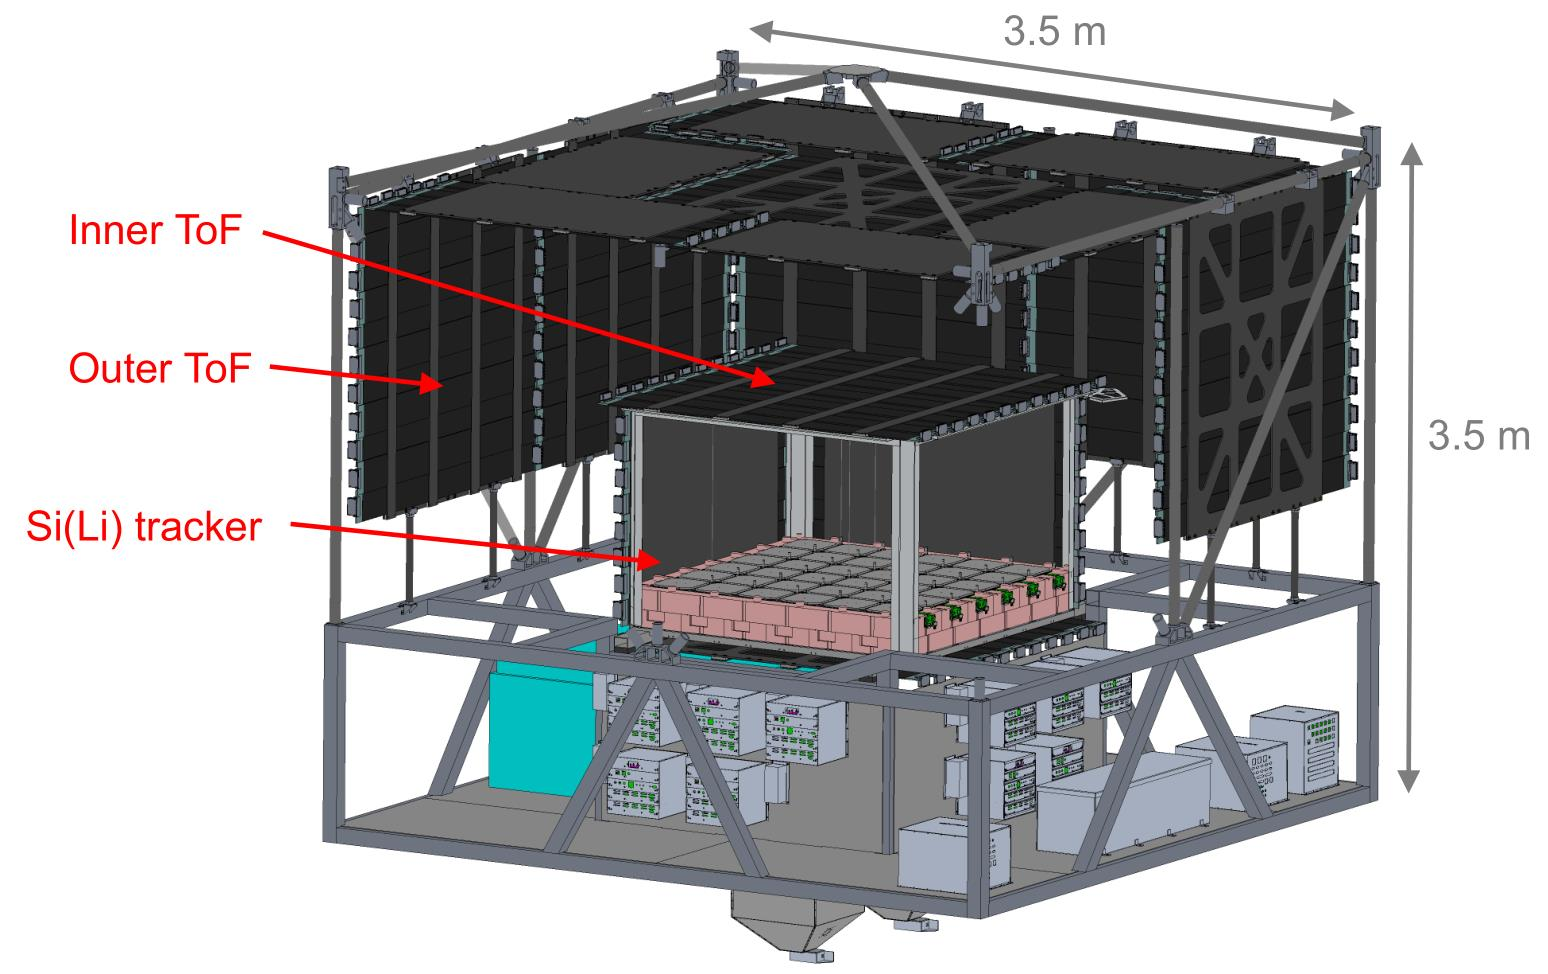
\includegraphics[width=0.9\textwidth]{Images/appendGAPSintro/GAPS_tracker_structure.jpg}
    \caption{Complete GAPS tracking system structure.}
    \label{figGAPStrackerstructure}
\end{figure}

%-------------------------------------------------------------------------------

\subsection*{GAPS tracking system}
\label{gapsTrackingSystem}
The GAPS instrument, shown in \hyperref[figGAPStrackerstructure]{Figure \ref{figGAPStrackerstructure}}, is mainly composed of \cite{rogers_2019_largearea}:

\begin{itemize}
    \itemsep0em
    \item Two external layers of TOF plastic scintillators that surround the inner tracker. The outer TOF dimension are $3.5 \times \SI{3.5}{\metre\squared}$, with an height of \SI{1.5}{\metre}. The inner TOF dimension are $1.5 \times \SI{1.5}{\metre\squared}$, with height of \SI{1}{\metre}. The distance between the outer TOF and the inner TOF is \SI{1}{\metre}. The entire TOF time resolution is about \SI{300}{\pico\second} \cite{doetinchem_2020_cosmicray}.
    \item The inner tracker, that is subdivided in 10 layers with \SI{10}{\cm} separation in order to achieve 3D particle tracking. Each layer is composed of $12 \times 12$ Si(Li) detectors \cite{spieler_2014_semiconductor}. Each detector has a diameter of \SI{10}{\cm} and a thickness of \SI{2.5}{\mm}. Moreover, each detector is segmented in eight strips in order to improve the spatial resolution enough to distinguish tracks from incident particles and exotic atom annihilation products. Each strip is then connected to a front-end channel which processes the charge released by the passing particle. The GAPS detectors are capable to detect X-rays ranging from \SI{20}{\kilo\electronvolt} to \SI{80}{\kilo\electronvolt} and charged particles up to \SI{50}{\mega\electronvolt}, at an operating temperature of \SI{-40}{\celsius}, with a FWHM energy resolution lower than \SI{4}{\kilo\electronvolt}. During flight, the cooling operation will be executed by a passive oscillating heat pipe approach, tested on two prototype test flights \cite{okazaki_2014_development}.
    \item As regards the electronics, each layer of the inner tracker is composed of $6 \times 6$ modules. Each module is made of one readout ASIC and one front-end board. 4 detectors are connected to one module. Each ASIC consists of 32 front-end channels capable to process the signals coming from 32 strips. The front-end board includes all the components used to guarantee the correct functionality of the ASIC. Two front-end boards can be connected with a flex-rigid board, specifically designed for this task, for a maximum of six front-end boards connected on the same line.
\end{itemize}

%-------------------------------------------------------------------------------
%   GAPS front-end
%-------------------------------------------------------------------------------

\section{GAPS front-end}
\label{secGAPSfrontend}

The final ASIC for the GAPS experiment, called SLIDER32, has 32 channels. Each channel is connected to one strip of the detector. When an antiparticle passes through one strip of the GAPS instrument, it loses energy in each layer of the Si(Li) detectors. When it has lost enough energy, it stops and forms an exotic excited atom. Finally, the atom de-excites and emits X-rays. The remaining nucleus annihilates, emitting pions and protons. When an antiparticle passes through a strip of the detector, it releases a certain amount of charge. 

\par
The product of the antiparticle annihilation release a certain amount of charge in the detector strips. The channel front-end main goal is to evaluate this amount of charge, coming from the corresponding strip of the detector. This is obtained by collecting the current pulses, at the input of the channel, and converting them into an analog voltage, which is subsequently digitised by an analog-to-digital converter. From these digitised values it is possible to understand which particle passed through the detector. 

\par
The GAPS front-end channel has been designed with a \SI{180}{\nano\meter} CMOS technology and its schematic is shown in \hyperref[figGAPSchannel]{Figure \ref{figGAPSchannel}}. The design has been carried out to target the experiment requirements reported in \hyperref[tabGAPSrequirements]{Table \ref{tabGAPSrequirements}}.

\begin{table}[ht]
    \centering
    %\def\arraystretch{1.3}
    \begin{tabular}{c c} 
         \Xhline{2\arrayrulewidth}
         Requirement & Value \T\B \\
         \hline
         Temperature & \SI{-40}{\celsius} \T\B \\
         Power consumption & < \SI{10}{\milli\watt}/channel \T\B \\
         Input dynamic range & \SI{10}{\kilo\electronvolt} - \SI{50}{\mega\electronvolt} \T\B \\
         Maximum electronic noise interference & \SI{4}{\kilo\electronvolt} (FWHM) \T\B \\
         Minimum threshold & \SI{10}{\kilo\electronvolt} \T\B \\
         Detector leakage current & max \SI{50}{\nano\ampere} @ \SI{27}{\celsius} \T\B \\
         \Xhline{2\arrayrulewidth}
    \end{tabular}
    \caption{GAPS ASIC requirements.}
    \label{tabGAPSrequirements}
\end{table}


%-------------------------------------------------------------------------------

\subsection*{Injection circuit}
The injection circuit generates a current pulse, whose amplitude is decided by the user, in order to simulate the release of charge due to the passage of particles through the GAPS Si(Li) detector. This block is used only during the test phase, because in the real experiment, the channels will be connected to the detector stripes. 

\par
An injection capacitor $C_{inj}$, shown in \hyperref[figGAPSchannel]{Figure \ref{figGAPSchannel}}, is integrated in each channel to generate the current pulse emulating the charge released in the detector.

\begin{figure}[h!]
    \centering
    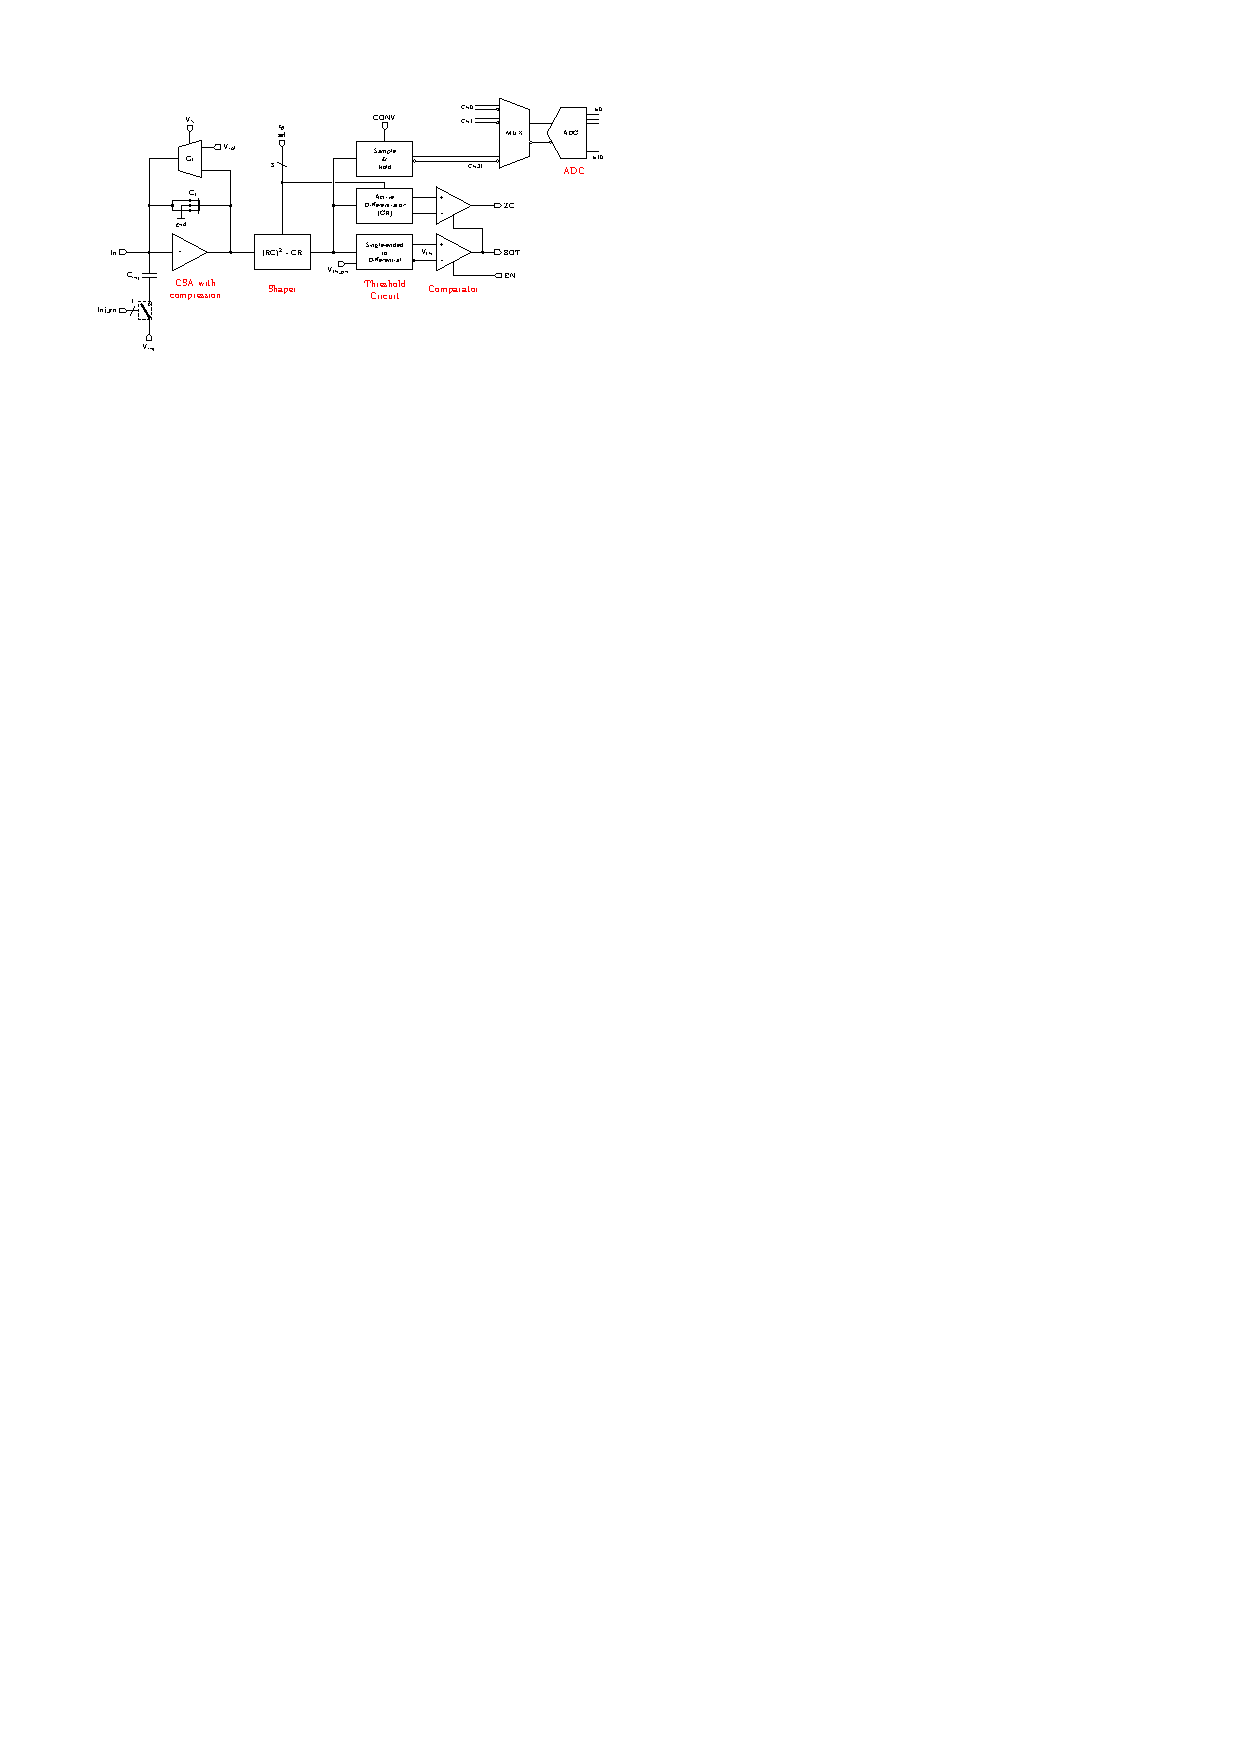
\includegraphics[width=0.98\textwidth]{Images/appendGAPSintro/readoutchannelADC.pdf}
    \caption{Front-end channel schematic.}
    \label{figGAPSchannel}
\end{figure}

%-------------------------------------------------------------------------------

\subsection*{Charge Sensitive Amplifier with dynamic signal compression}
The first block of the channel is the Charge Sensitive Amplifier. The aim of this block is to convert the current pulses coming from the detector into a voltage step, whose amplitude is proportional to area of the current pulse. The main feature of this block is its input-output trans-characteristic, which is characterised by signal dynamic compression. This a very important feature of the CSA because, in order to cover the large energy dynamic range required by the project specifications and to maintain a high resolution in the low energy range, a linear gain was not an option due to the high supply voltage and large number of bits required for this solution.

\par
The CSA has been designed with an active folded cascode (with a local feedback) loaded by an active cascode architecture. The reset is performed by a continuous time feedback implemented with a Krummenacher network. The dynamic compression has been performed using the nMOS capacitor $C_f$.

%-------------------------------------------------------------------------------

\subsection*{Time-invariant filter (CR-(RC)\textsuperscript{2})}
\label{shaper}
The second block of the GAPS channel is the shaper. This block’s main goal is to improve the Signal-to-Noise ratio in order to obtain the required high energy resolution. It is composed of two stages: one CR stage (high-pass filter) and two RC stage (low-pass filter). The Transfer Function of this block is

\begin{equation}
    H(s) = \frac{R_2}{R_1} \cdot \frac{1}{1+s\tau} \cdot \frac{C_2}{C_1} \cdot \frac{s\tau}{(1+s\tau)^2}
\end{equation}

\noindent
The shaper output is a unipolar semi-Gaussian function, characterized by a peaking time $t_p = 2 \cdot \tau$, where $\tau$ is the time constant of the circuit. The peaking time selection (3 bit) is obtained by switching four capacitors $C_1$, $C_2$, $C_p$ and $C_i$. The shaper output introduces a gain of 1.5 almost independent of the peaking time.

%-------------------------------------------------------------------------------

\subsection*{Threshold Generator and SOT comparator} \label{thrSOT}
The shaper output is connected to the threshold generator. The other two inputs are two threshold voltages called $V_{tp}$ and $V_{tn}$. This block converts the single-ended signal at the output of the shaping stage to a differential signal. A differential threshold voltage is used to avoid crosstalk. The two output signals of the threshold generator are:

\begin{equation}
    V_{th, out1} = v_{s0} + V_{tp} - \frac{V_{sh}}{2}
\end{equation}

\begin{equation}
    V_{th, out2} = v_{s0} + V_{tp} - \frac{V_{sh}}{2}
\end{equation}

\noindent
where $V_{sh}$ is the shaper output voltage and $v_{s0}$ is a threshold generator bias voltage. The differential signal obtained is

\begin{equation}
    \begin{split}
        V_{th, out1} - V_{th, out2} & = (v_{s0} + V_{tp} - \frac{V_{sh}}{2}) - (v_{s0} + V_{tn} + \frac{V_{sh}}{2}) \\
        & = V_{tp} - V_{tn} - V_{sh}
    \end{split}
\end{equation}

The difference $(V_{tp} - V_{tn})$ can be expressed as $V_{th}$, which is the SOT comparator threshold. The two generated voltages are, in fact, connected to the SOT comparator. Its main goal is to suppress false event caused by noise or disturbances. The comparator fires when

\begin{equation}
    V_{th, out2} > V_{th, out1}
\end{equation}

\noindent
or, more easily, when

\begin{equation}
    V_{sh} > V_{th}
\end{equation}

\noindent
In the SLIDER32 ASIC, $V_{tp}$ and $V_{tn}$ are generated by means of an 8-bit DAC external to the channels. These voltages are then connected to the threshold generator of each channel. In order to compensate for process parameter variations of each channel threshold, in each one of these a 3-bit DAC for fine threshold trimming is added.

%-------------------------------------------------------------------------------

\subsection*{Active CR differentiator and Zero Crossing comparator (ZC)}
\label{zeroCrossing}

The differentiator task is to derive the shaper output, with a CR filter, in order to detect the exact shaper peaking time. When the shaper signal derivative is equal to zero, the shaper output is at its maximum voltage, namely its peaking time. The differentiator output is negated by this block and, in this process, a continuous voltage of $V_{dd}/2$ is added to the derivative signal. This voltage addition prevents that, if the derivative is less than \SI{0}{V}, the differentiator output will be always at \SI{0}{V}. The output of this block is then connected to the ZC comparator and compared with $V_{dd}/2$ voltage: when its voltage is greater than $V_{dd}/2$, the ZC output turns into a logic 1. This is the time when the shaper output has to be sampled, throughout the \texttt{CONV} signal, in order to retrieve the exact injected charge. 

\par
The ZC comparator works only if the SOT comparator voltage is at logic 1. This is done in order to easily discard false events caused by noise or external disturbances.

%-------------------------------------------------------------------------------

\subsection*{Single-ended to differential S\&H}
This block holds the shaper output voltage value when the signal \texttt{CONV} passes from logic 0 to logic 1. The \texttt{CONV} signal is equal to ZC when the front-end operates in self-trigger mode, instead, when it operates in non self-trigger mode, the \texttt{CONV} signal must be provided from an external source.

\par
The sample \& hold output is then connected to a multiplexer, and finally to an ADC used to digitise to voltage stored in it. All the blocks signals are shown in \hyperref[figASICsignals]{Figure \ref{figASICsignals}} for an incoming energy of \SI{100}{\kilo\electronvolt} at \SI{-40}{\celsius}.

\begin{figure}[h!]
    \centering
    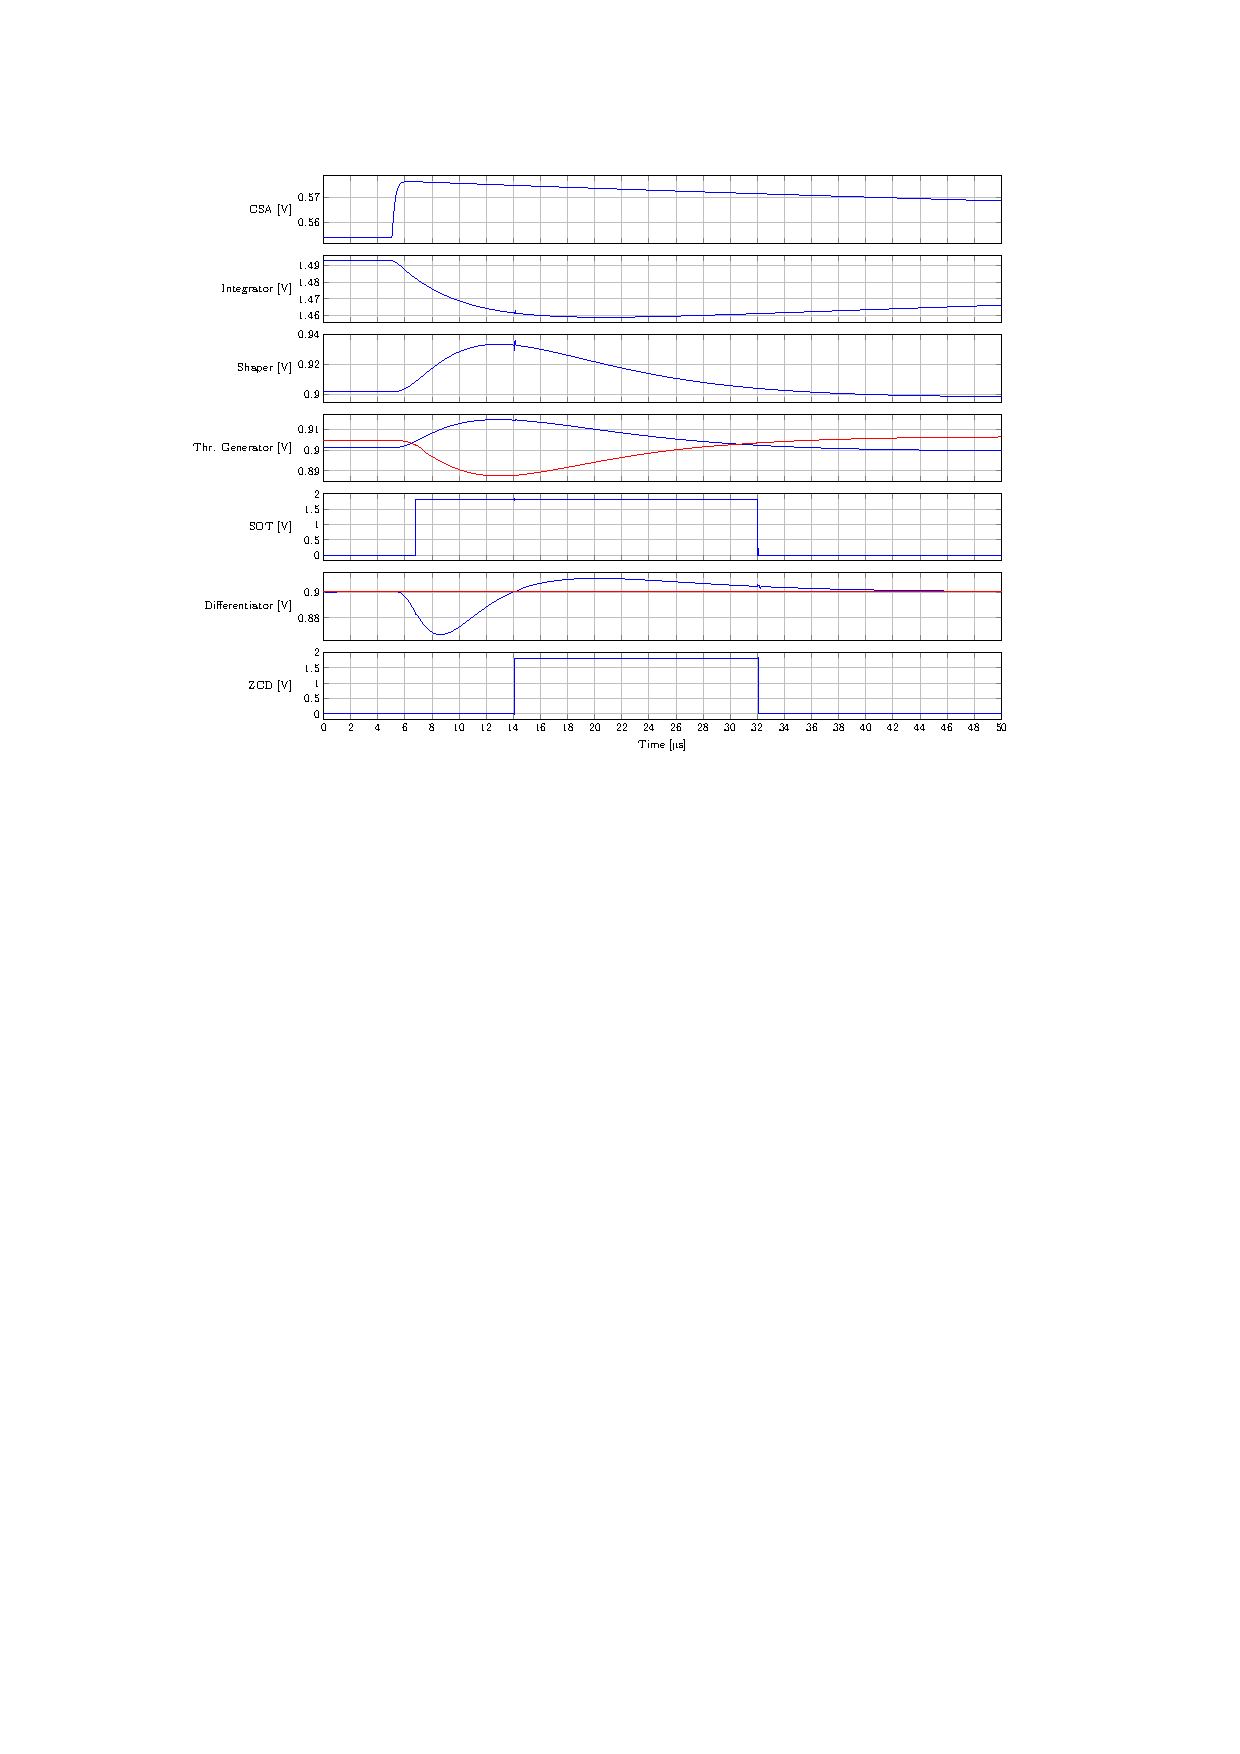
\includegraphics[width=0.9\textwidth]{Images/appendGAPSintro/ASIC_riassunto_segnali.pdf}
    \caption{All channel blocks signals for an incoming energy of \SI{100}{\kilo\electronvolt} at \SI{-40}{\celsius}.}
    \label{figASICsignals}
\end{figure}
